\documentclass[]{exam}
\usepackage[utf8]{inputenc}
\usepackage{enumitem}
\usepackage{amsmath}
\usepackage{amsfonts}
\usepackage{setspace}
\usepackage{verbatim} 
\usepackage{graphicx} 
\usepackage{gensymb}
\usepackage{color}
\usepackage{commath}
\usepackage{fancyvrb}
\doublespacing
\graphicspath{{C:\Users\Johnnia\Desktop\常用\Spring2017\CSE 373\HW5}}
\title{}

%===> Formatting ===>
\setlength{\parskip}{8pt}
\setlength{\parindent}{20pt}
%<=== Formatting <===


\title{CSE 373 HW5 Write Up}
\author{Chongyi Xu}

\begin{document}
	
\maketitle
\begin{questions}

\question \textbf{Topological Sort:} Determine a topological ordering for the following directed acylic graph. Show your work 
\\
\begin{tabular}{ c c c c c c c c }
 					&A 					& B 			& C 			& D 				& E 				& F 		& G \\ 
 removed& x 	& x 			& x 			& x 				& x 				& x 		& x \\  
 degree	& 0 	& $\not 1$ 0 	& $\not 1$ 0	& $\not 2\ \not 1$ 0& $\not 2\ \not 1$ 0&$\not 1$ 0	& 0
\end{tabular}
\\ One possible ordering will be [A, G, F, B, D, E, C]

\question \textbf{Minimum Spanning Algorithm:} Use the following graph for both of the following minimum spanning tree algorithms.
\begin{parts} 
\part Build a minimum spanning tree for the graph using Kruskals algorithm. Number each edge according to when it is entered into the minimum spanning tree. THe first edge will get number 1, etc. Show the ordering of the edges you consider by showing the state of the pending set of edges to consider.
\\
\\ Edges in sorted order:
\\ cost 1: (B, E) (D, G) (C, G)
\\ cost 2: (A, B) (E, F) (C, D)
\\ cost 3: (B, F) (A, E) (E, G)
\\ cost 4: (A, D) (F, G)
\\
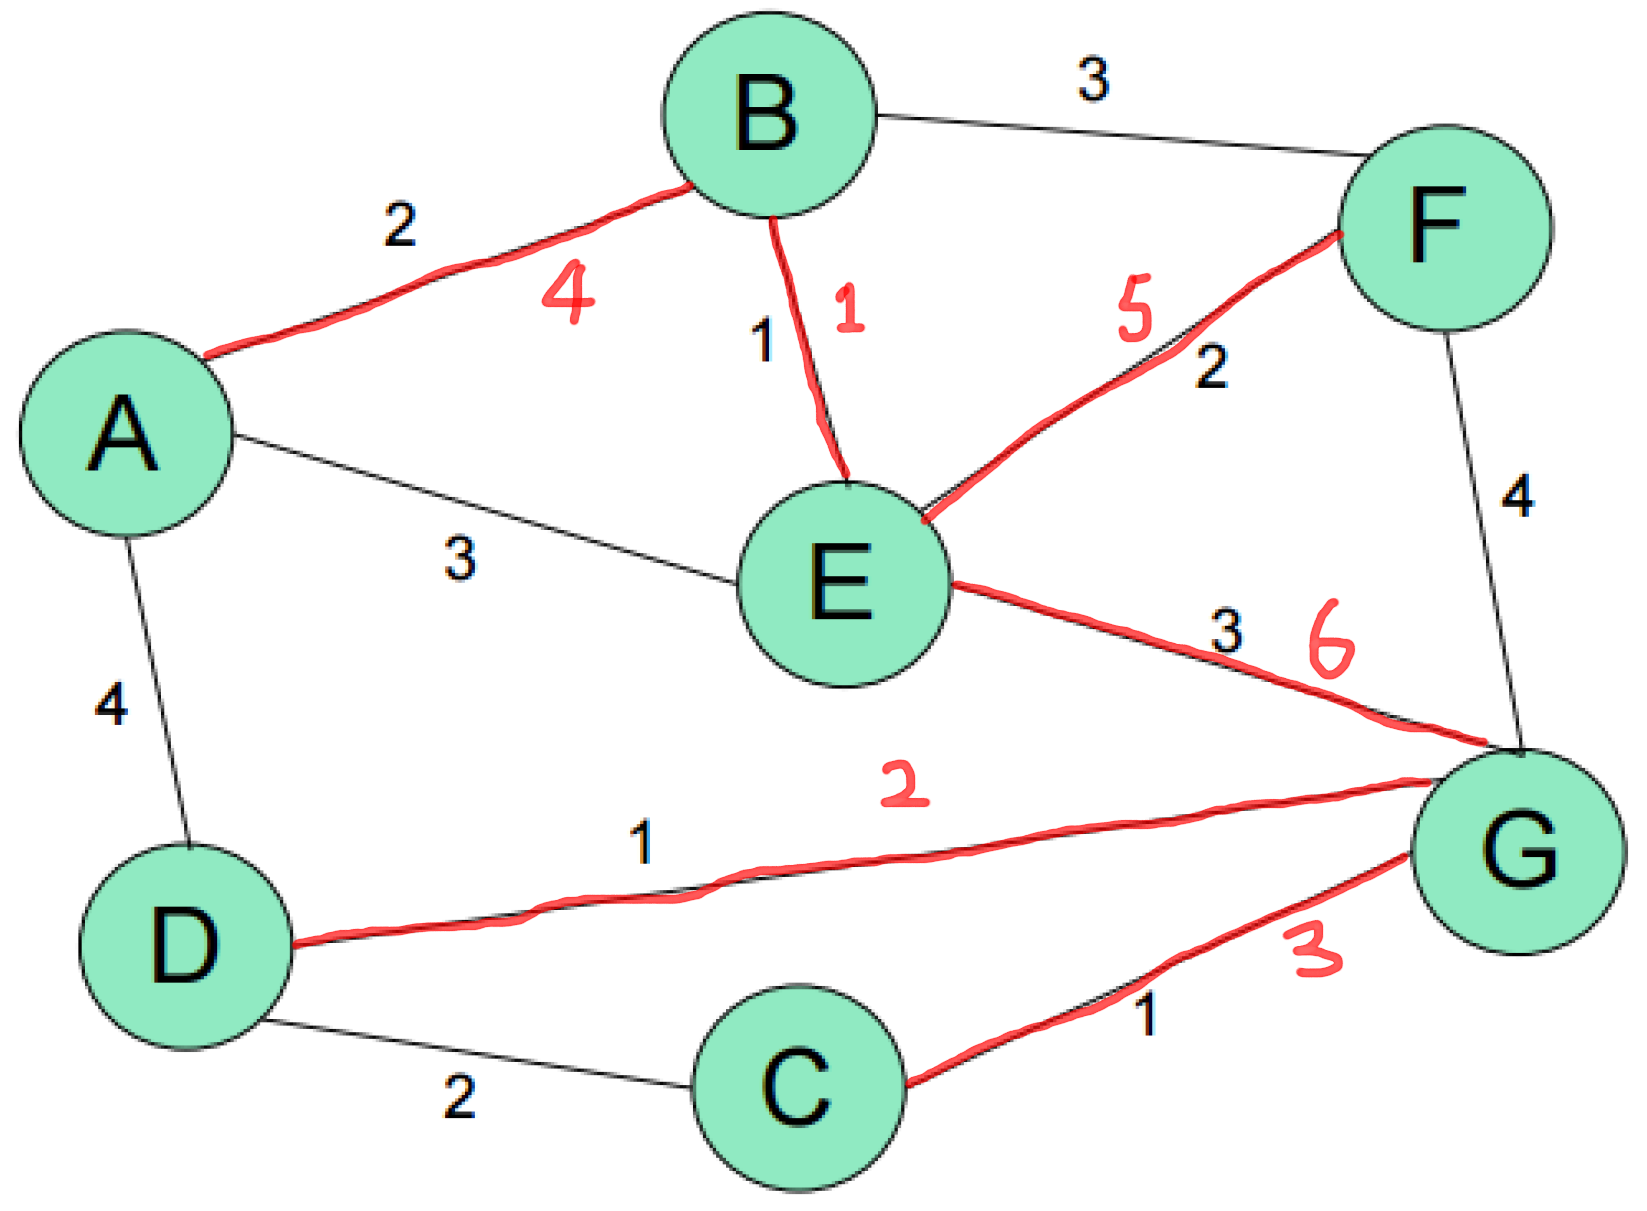
\includegraphics[scale = 0.2]{Kruskals.png}
\\ So the ordering will be [(B, E), (D, G), (C, G), (A, B), (E, F), (E, G)]
\part Now build a MST for the graph using Prims algorithm, starting with vertex A.
\\
\begin{tabular} {c c c c}
	& known?		& cost 			& previous \\
A 	& \checkmark	& 0				&	 \\
B 	& \checkmark	& 2 			& A \\
C 	& \checkmark	& 1 			& G \\
D 	& \checkmark 	& $\not 4$ 1	& $\not A$ G \\
E 	& \checkmark 	& $\not 3$ 1	& $\not A$ B \\
F 	& \checkmark 	& $\not 3$ 2	& $\not B$ E \\
G 	& \checkmark 	& 3 			& E
\end{tabular}
\\
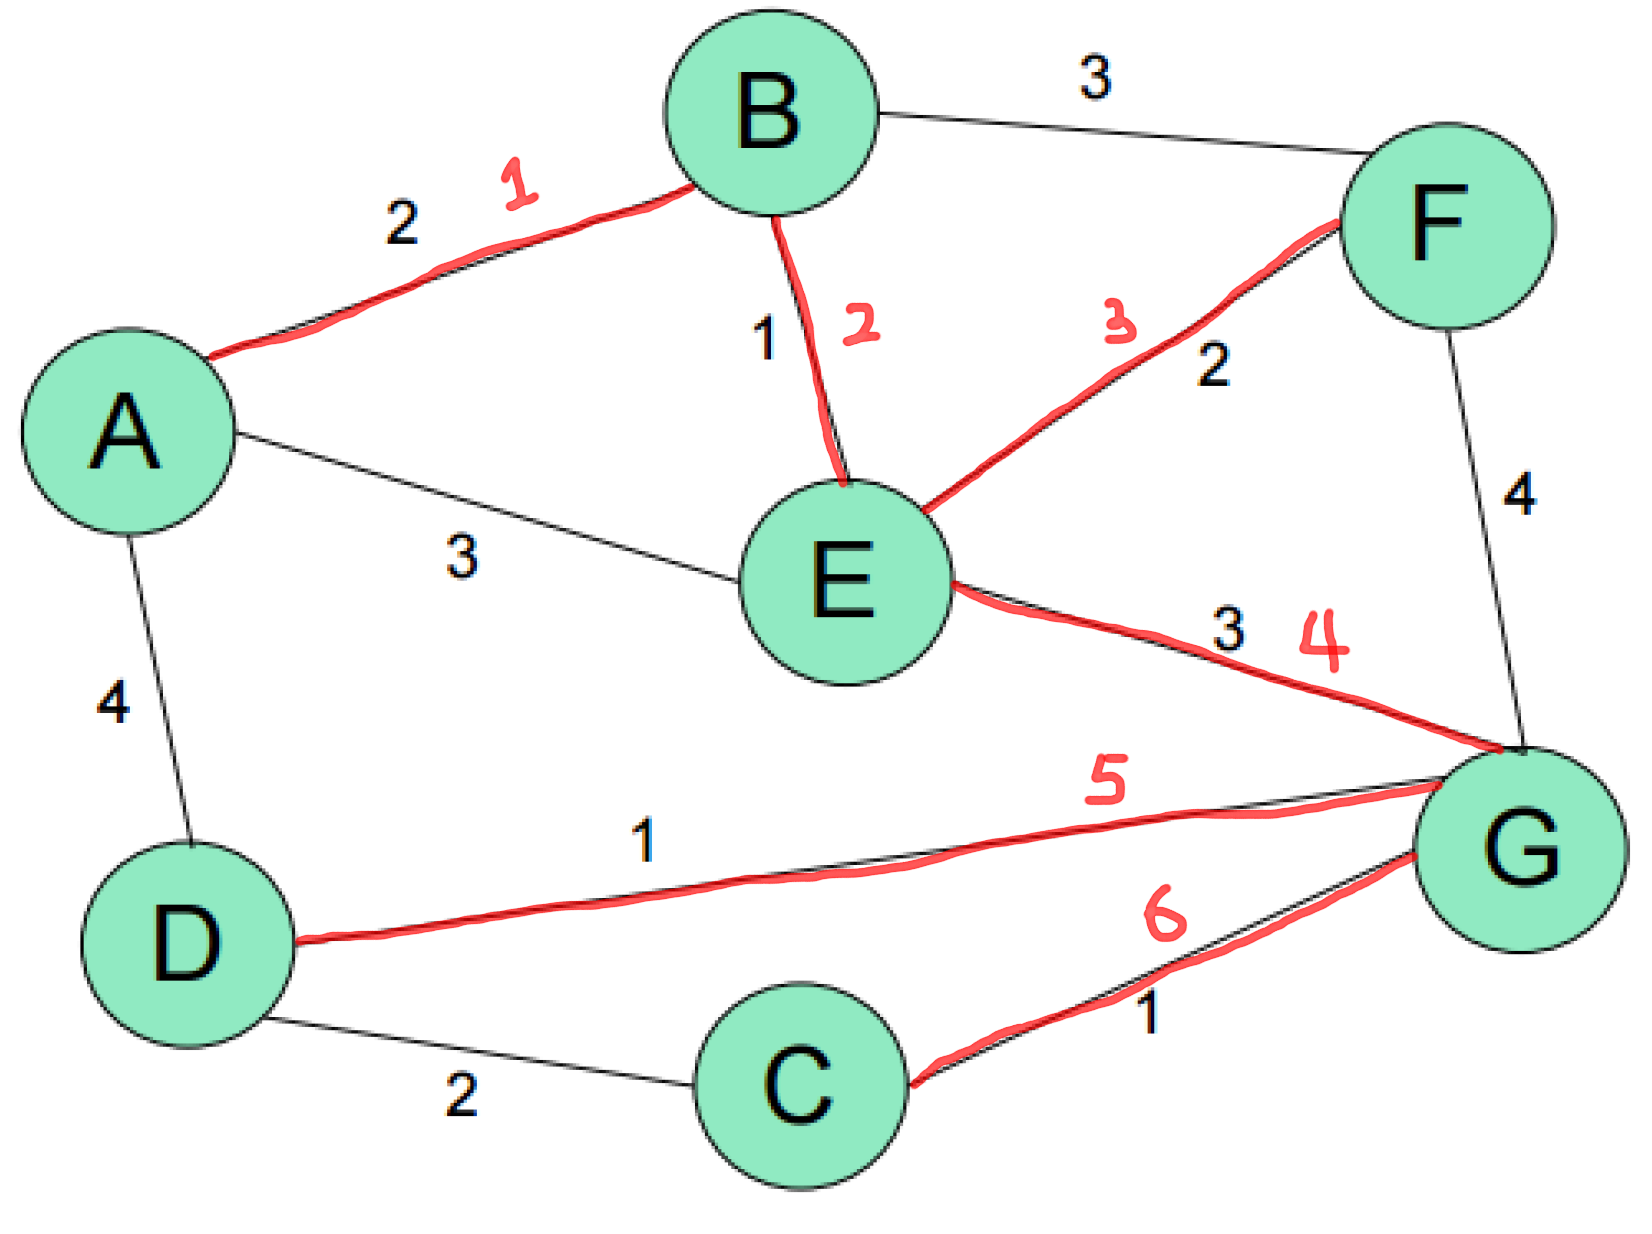
\includegraphics[scale = 0.2]{Prim.png}
\end{parts}

\question \textbf{Dijkstra's and Negative Edges:}
\begin{parts}
\part If there is more than one minimum cost path from v to w, will Dijkstra's Algorithm always find the path with the fewest edges? If not, explain in a few sentences how to modify Dijkstra's Algorithm so that if there is more than one minimum path from v to w, a pth with the fewest edges is chosen. Assume no negative weight edges or negative weight cycles.
\\ It will not always find the shortest path since when we are comparing costs, we just compare the value without considering the number of edges. If the costs are the same, the second path will be ignored. If we would like to compare the number of edges, we could make a field to keep track of the least number of edges. And every time we find two paths with the same cost, we could then compare the number of edges to decide which path we should pick.

\part Given an example where Dijkstra's Algorithm gives the wrong answer in the presence of a negaive cost edge but no negative-cost cycles. 
\\ 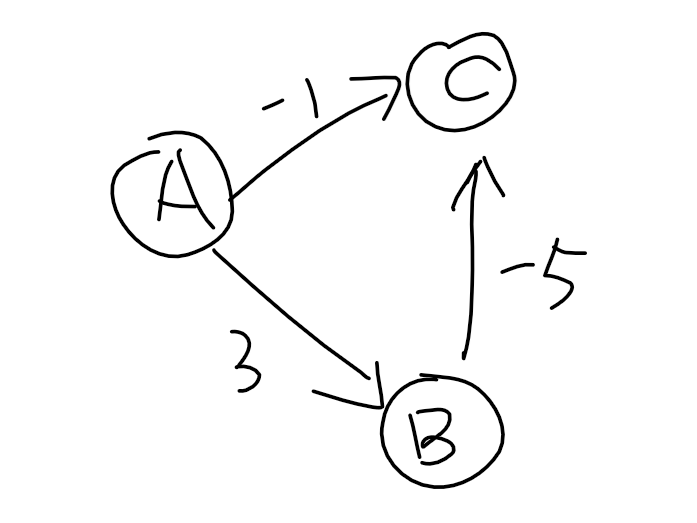
\includegraphics[scale = 0.5]{example.png}
\\ In this case, we first check \textbf{C} as known with cost -1, then we check \textbf{B} as known with cost 3. But after we check \textbf{B}, we find another path to \textbf{C} which has a lower cost comparing to what we have assigned to \textbf{C}, which is -2. So Dijkstra's Algorithm fails here. 
\part Suppose you are given a graph that has negative-cost edges but no negative-cost cycles. Consider the following strategy to find shortest paths in this graph: Uniformly add a constant k to the cost of every edge, so that all costs become non-negative, then run Dijstra's Algorithm and return that result with the edge costs reverted back to their original values.
\\ 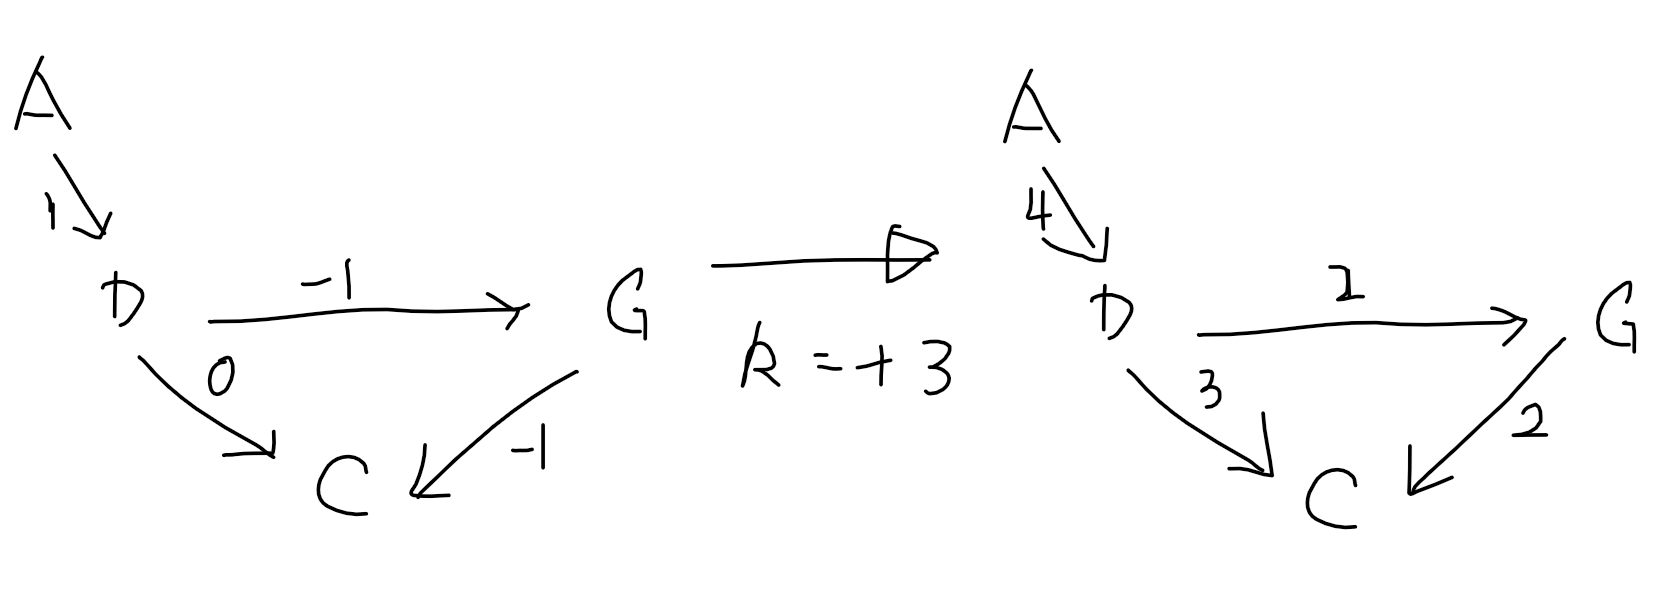
\includegraphics[scale = 0.2]{example2.png}
\\ This method fails in this case when we want to find the shortest path from \textbf{A} to \textbf{C}. In the original graph (with negative-cost edges), the shortest path will be $\textbf{A}\to\textbf{D}\to\textbf{G}\to\textbf{C}$ with cost -1, but after the transformation, the shortest path will be $\textbf{A}\to\textbf{D}\to\textbf{C}$ with cost 7.
\\ In general, it fails because the transformation is adding a constant to every edge, which means the path with more edges will have a greater increasement rather than the one with less edges.
\end{parts}

\question Describe how you tested your \verb|shortestPath| method. Explain any difficulties in implementation you may have experinced and how testing helped find the problem, if applicable.
\\ Firstly, I draw the graph to have a clear image of what am I testing. 
\\ 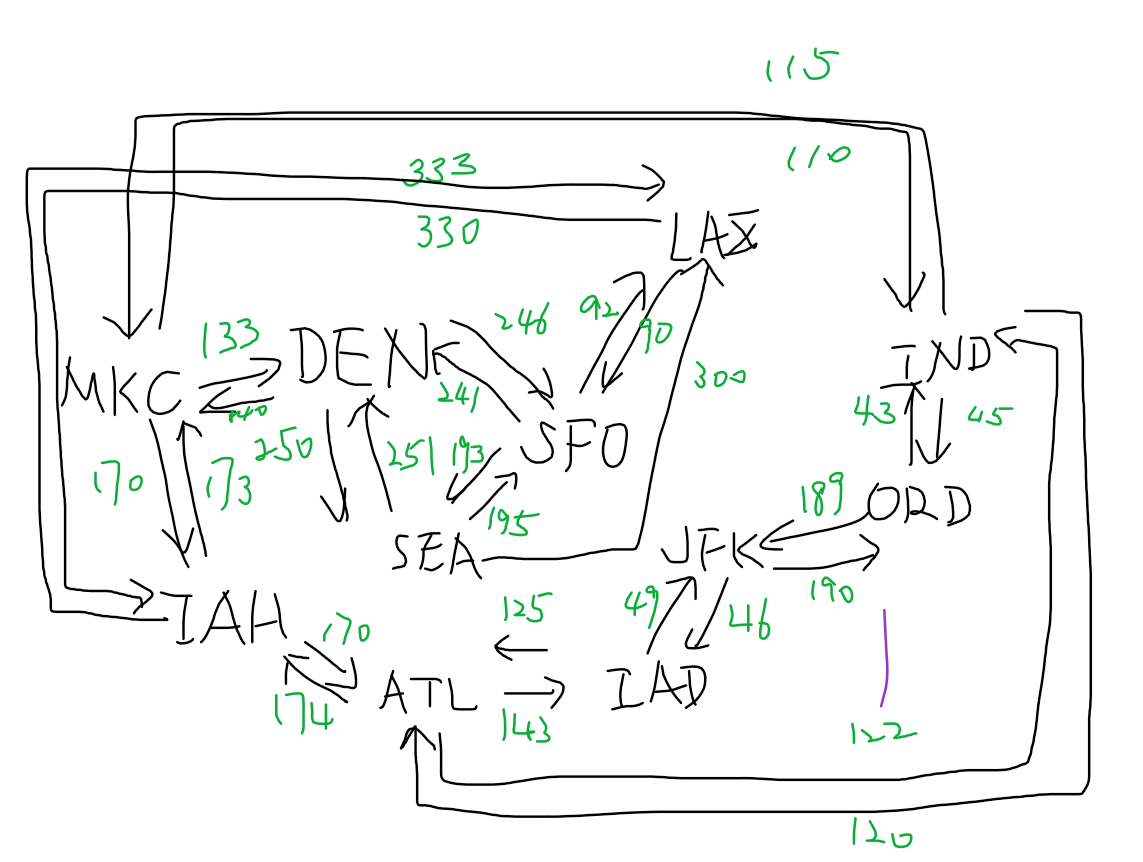
\includegraphics[scale = 0.3]{Dij.png}
\\ Then I do a lot of tests. In particulr, I tested the following special cases:
\begin{itemize}
	\item When the start point and the destination point are the same
	\item Make multiple times of different calls to check if the original data is not changed
	\item Try different start points
\end{itemize}
\begin{Verbatim}
Path shortest = g.shortestPath(a, b);
if (shortest == null) {
	System.out.println(a.toString() + " is not reachable from " + b.toString());
} else {
	System.out.println("The least cost will be " + shortest.cost);
	System.out.println("The shortest path will be " + shortest.vertices.toString());
}
\end{Verbatim}
As I tested my \verb|shortestPath| method, I found out that my code does not successfully keep the original data(vertices) unchanged. This problem was found when I tried call two times of \verb|shortestPath| method, the second time gave me the wrong path. Then I went back to my method and created another container(vertex) to do Dijkstra's Algorithm. In such way, my original data will not be changed so that I could make multiple calls.


\end{questions}
\end{document}
